\documentclass[a4paper,
fontsize=11pt,
%headings=small,
oneside,
numbers=noperiodatend,
parskip=half-,
bibliography=totoc,
final
]{scrartcl}

\usepackage[babel]{csquotes}
\usepackage{synttree}
\usepackage{graphicx}
\setkeys{Gin}{width=1\textwidth} %default pics size

\graphicspath{{./plots/}}
\usepackage[ngerman]{babel}
\usepackage[T1]{fontenc}
%\usepackage{amsmath}
\usepackage[utf8x]{inputenc}
\usepackage [hyphens]{url}
\usepackage{booktabs} 
\usepackage[left=2.4cm,right=2.4cm,top=2.3cm,bottom=2cm,includeheadfoot]{geometry}
\usepackage{eurosym}
\usepackage{multirow}
\usepackage[ngerman]{varioref}
\setcapindent{1em}
\renewcommand{\labelitemi}{--}
\usepackage{paralist}
\usepackage{pdfpages}
\usepackage{lscape}
\usepackage{float}
\usepackage{acronym}
\usepackage{eurosym}
\usepackage{longtable,lscape}
\usepackage{mathpazo}
\usepackage[normalem]{ulem} %emphasize weiterhin kursiv
\usepackage[flushmargin,ragged]{footmisc} % left align footnote
\usepackage{ccicons} 
\setcapindent{0pt} % no indentation in captions

%%%% fancy LIBREAS URL color 
\usepackage{xcolor}
\definecolor{libreas}{RGB}{112,0,0}

\usepackage{listings}
\usepackage{tabularx}

\urlstyle{same}  % don't use monospace font for urls

\usepackage[fleqn]{amsmath}

%adjust fontsize for part

\usepackage{sectsty}
\partfont{\large}

%Das BibTeX-Zeichen mit \BibTeX setzen:
\def\symbol#1{\char #1\relax}
\def\bsl{{\tt\symbol{'134}}}
\def\BibTeX{{\rm B\kern-.05em{\sc i\kern-.025em b}\kern-.08em
    T\kern-.1667em\lower.7ex\hbox{E}\kern-.125emX}}

\usepackage{fancyhdr}
\fancyhf{}
\pagestyle{fancyplain}
\fancyhead[R]{\thepage}

% make sure bookmarks are created eventough sections are not numbered!
% uncommend if sections are numbered (bookmarks created by default)
\makeatletter
\renewcommand\@seccntformat[1]{}
\makeatother

% typo setup
\clubpenalty = 10000
\widowpenalty = 10000
\displaywidowpenalty = 10000

\usepackage{hyperxmp}
\usepackage[colorlinks, linkcolor=black,citecolor=black, urlcolor=libreas,
breaklinks= true,bookmarks=true,bookmarksopen=true]{hyperref}
\usepackage{breakurl}

%meta
%meta

\fancyhead[L]{N. Haupka, N. Jahn, A. Hobert\\ %author
LIBREAS. Library Ideas, 41 (2022). % journal, issue, volume.
\href{https://doi.org/10.18452/24800}{\color{black}https://doi.org/10.18452/24800}
{}} % doi 
\fancyhead[R]{\thepage} %page number
\fancyfoot[L] {\ccLogo \ccAttribution\ \href{https://creativecommons.org/licenses/by/4.0/}{\color{black}Creative Commons BY 4.0}}  %licence
\fancyfoot[R] {ISSN: 1860-7950}

\title{\LARGE{Praxisbericht Big Scholarly Data an der SUB Göttingen}}% title
\author{Nick Haupka, Najko Jahn, Anne Hobert} % author

\setcounter{page}{1}

\hypersetup{%
      pdftitle={Praxisbericht Big Scholarly Data an der SUB Göttingen},
      pdfauthor={Nick Haupka, Najko Jahn, Anne Hobert},
      pdfcopyright={CC BY 4.0 International},
      pdfsubject={LIBREAS. Library Ideas, 41 (2022)},
      pdfkeywords={Big Scholarly Data, Bibliometrie,Open Access Transformation,Hybrides Open Access},
      pdflicenseurl={https://creativecommons.org/licenses/by/4.0/},
      pdfcontacturl={http://libreas.eu},
      baseurl={},
      pdflang={de},
      pdfmetalang={de},
      pdfdoi={10.18452/24800},
      pdfurl={https://doi.org/10.18452/24800}
     }
   
   



\date{}
\begin{document}

\maketitle
\thispagestyle{fancyplain} 

%abstracts
\begin{abstract}
\noindent
Der Beitrag stellt den Einsatz des kommerziellen
Cloud-Computing-Dienstes Google BigQuery für die Arbeit mit großen
offenen Datensätzen über wissenschaftliche Veröffentlichungen an der
Niedersächsischen Staats- und Universitätsbibliothek Göttingen (SUB
Göttingen) vor, insbesondere bezogen auf den Datenbestand, die
Prozessierung und die Zugriffsmöglichkeiten. Als beispielhafter Use Case
werden überregionale Open-Access-Transformationsverträgen in Deutschland
bezogen auf ihren Open-Access-Anteil analysiert.
\end{abstract}

%body
\hypertarget{motivation}{%
\section{Motivation}\label{motivation}}

An der Niedersächsischen Staats- und Universitätsbibliothek Göttingen
(SUB Göttingen) führen wir als Data-Analysis-Team für Wissenschaftliche
Information regelmäßig Analysen von Daten über wissenschaftliche
Publikationen durch. Dabei untersuchen wir Fragestellungen im
Zusammenhang bibliometrischer Forschungsprojekte, wollen aber auch
datengestützte strategische Entscheidungen an unserer Universität und
darüber hinaus ermöglichen.

Unser Augenmerk liegt auf frei verfügbaren großen Datensätze über
wissenschaftliche Informationsprozesse, sogenannte Big Scholarly Data.
Deren Offenheit ermöglicht es uns, ohne hohe Investitionskosten etwa für
die Lizenzierung einer Datenquelle Analysen durchzuführen. Offene Daten
erhöhen zudem die Transparenz unserer Analysen, da wir sowohl Daten als
auch Analysecode gemeinsam mit unseren Berichten offen verfügbar machen
können. Zudem sind wir ein kleines Team und daher auf die Zusammenarbeit
mit Kolleg*innen anderer Einrichtungen angewiesen, mit denen wir
jederzeit auf den gleichen Datenpool zugreifen können, was mit offenen
Daten prinzipiell möglich ist.

Bei unserer Arbeit mit Big Scholarly Data hat sich schnell
herausgestellt, dass wir einen verteilten und hochperformanten Zugriff
benötigen. Große Datensätze über wissenschaftliche Publikationen werden
hauptsächlich als (unbearbeitete, nicht vollständig strukturierte)
Datendumps bereitgestellt, deren lokale Prozessierung sehr aufwendig und
wegen fehlender Rechenkapazitäten nur bedingt möglich ist. Wichtig war
uns zudem, auch ohne ausgeprägte Kenntnisse der Datenbank- und
Serveradministration, gemeinsam Datenanalysen durchführen zu können. Aus
diesem Grunde verwenden wir die Cloud-basierte Datenbankumgebung Google
BigQuery, ein serverloses Data Warehouse für die hochperformante Analyse
großer Datenbestände.\footnote{\url{https://cloud.google.com/bigquery?hl=de}}

Begonnen haben wir mit Google BigQuery im Jahr 2019, und zwar mit dem
Download und der Prozessierung der Datensnapshots des
Open-Access-Discovery-Services Unpaywall\footnote{\url{https://unpaywall.org/}}.
Die Snapshots haben wir im Rahmen des BMBF-Forschungsprojekts
OAUNI\footnote{\url{https://www.wihoforschung.de/wihoforschung/de/bmbf-projektfoerderung/foerderlinien/quantitative-wissenschaftsforschung/oauni/oauni_node.html}}
aufbereitet, um Unpaywall dahingehend zu analysieren, welche
Informationen zum Open-Access-Status wissenschaftlicher Publikationen in
der Datenquelle enthalten sind.\footnote{Siehe zum Beispiel Jahn et
  al.~(2021) und Hobert et al.~(2021).} Mit der Zeit konnten wir unsere
Routinen zur Datenaufbereitung verfeinern und unser Portfolio durch
Hinzunahme zusätzlicher Datenquellen wie Crossref oder OpenAlex
erweitern.

Im Beitrag beschreiben wir, wie wir mit Google BigQuery arbeiten,
insbesondere den Datenbestand, die Prozessierung und die
Zugriffsmöglichkeiten. Zur Illustration geben wir einen kurzen Einblick
in die aktuelle Entwicklung von Dashboards zur Wirksamkeit von
Transformationsverträgen in Deutschland, die wir im Rahmen eines
DFG-Projekts zur Kostentransparenz des Lizenzmodells entwickeln.

\hypertarget{verfuxfcgbare-daten-innerhalb-der-google-bigquery-instanz}{%
\section{Verfügbare Daten innerhalb der Google
BigQuery-Instanz}\label{verfuxfcgbare-daten-innerhalb-der-google-bigquery-instanz}}

Unsere BigQuery-Instanz umfasst im Wesentlichen drei Datenquellen, die
wir pflegen und kuratieren: Unpaywall, Crossref und OpenAlex. Zu jeder
dieser Quellen existieren Schnittstellen, die es erlauben, einen
Snapshot der jeweiligen Datenquelle herunterzuladen. Die Snapshots
prozessieren wir entsprechend unserer datenanalytischen Anforderungen.
So liegt der Fokus unserer Arbeit häufig auf Veröffentlichungen in
wissenschaftlichen Journalen, weshalb wir oftmals keine kompletten
Snapshots in unsere Instanz überführen, sondern eine Teilmenge, die sich
auf Zeitschriftenartikel bezieht.

Unser BigQuery Data Warehouse ist dabei so aufgebaut, dass wir zu jeder
Quelle sowohl einen aktuellen (\emph{current}) als auch historische
(\emph{historical}) Snapshots anbieten. Historische Snapshots werden in
regelmäßigen Abständen (zum Beispiel jährlich) gesichert, sodass die
Entwicklung und Qualität einer Datenbank über einen zeitlichen Verlauf
beurteilt werden kann. Diese Snapshots verwenden wir auch für unsere
wissenschaftlichen Publikationen, da sie im Gegensatz zum regelmäßig
aktualisierten Datensatz (\emph{current}), niemals überschrieben werden.
Dadurch gewährleisten wir die Reproduzierbarkeit unserer Analysen. Der
jeweils aktuelle Snapshot (\emph{current}) benutzen wir in unseren
Dashboards und anderen Analysen, die einen möglichst aktuellen Bezug
erfordern und hauptsächlich die Bibliothekspraxis adressieren.

Die von uns bereitgestellten Snapshots können sich, wie angedeutet, von
den Snapshots der Datenbankanbieter leicht unterscheiden. So filtern wir
gezielt nach Zeitschriftenartikeln, entfernen Datenfelder und grenzen
das Publikationsvolumen auf bestimmte Jahre ein. Unsere bereitgestellten
Unpaywall-Snapshots enthalten beispielsweise nur Zeitschriftenartikel ab
2008, unsere Crossref-Tabellen hingegen Zeitschriftenartikel ab 2013.
Lediglich die OpenAlex-Snapshots befinden sich unverändert auf unserer
BigQuery-Instanz, da wir derzeit noch nicht einschätzen können, welche
Informationen in OpenAlex wir zukünftig auswerten möchten.

\hypertarget{prozessierung}{%
\subsection{Prozessierung}\label{prozessierung}}

Für jede der genannten Datenquellen haben wir eine Prozedur entwickelt,
die die Überführung eines Snapshots in BigQuery ermöglicht. Die dabei
angewandten Schritte lassen sich in Download,
Prozessierung/Transformation, Upload und Erstellung einer Tabelle in
BigQuery unterteilen.

Im ersten Schritt wird ein Big-Scholarly-Data-Snapshot auf Server der
Gesellschaft für wissenschaftliche Datenverarbeitung mbH Göttingen
(GWDG), die als Rechenzentrum der Universität Göttingen fungiert,
heruntergeladen. Im zweiten Schritt verwenden wir Skripte, die es
ermöglichen, die Datenbestände zu filtern, Datenfelder zu entfernen und
Zeittransformationen durchzuführen. Hiermit soll erreicht werden, dass
sich die Größe des Snapshots reduziert, wodurch wir
Cloud-Computing-Kosten sparen. Da die Snapshots meist sehr umfangreich
sind und mehrere hundert Gigabyte umfassen können, verwenden wir für die
Datentransformation das High Performance Cluster (HPC) der GWDG. Dieser
Service erlaubt es uns, durch die Bereitstellung leistungsstarker
Server, mit großen Datenmengen zu arbeiten. Je nach Konfiguration und
Datenbank kann die Transformation auf dem HPC mehrere Stunden dauern.
Das Resultat wird daraufhin in ein \enquote*{Google Bucket} geladen. Von
da aus kann eine Tabelle in BigQuery erstellt werden. Tabelle 1 zeigt
die von uns bereitgestellten Datenbanken sowie die angewendeten
Prozeduren.

Tabelle 1: Informationen zu den bereitgestellten Snapshots
\begin{longtable}[]{@{}
  >{\raggedright\arraybackslash}p{(\columnwidth - 4\tabcolsep) * \real{0.15}}
  >{\raggedright\arraybackslash}p{(\columnwidth - 4\tabcolsep) * \real{0.42}}
  >{\raggedright\arraybackslash}p{(\columnwidth - 4\tabcolsep) * \real{0.42}}@{}}
\toprule
Datenbank & Download & Prozedur \\
\midrule
\endhead
Unpaywall & Unpaywall-Snapshots werden in regelmäigen Abständen auf
einem Amazon S3 Cloud Storage angeboten. Die Snapshots sind in der Regel
zwischen 16 und 30 Gigabyte groß. Der Download ist kostenlos. Ein
Account wird nicht benötigt. & Bei der Prozessierung des Snapshots
verwenden wir das Command-Line-Tool jq
(\url{https://stedolan.github.io/jq/}) und das Programm parallel
(\url{https://www.gnu.org/software/parallel/}). Das von uns verwendete
Skript wird auf Github angeboten
(\url{https://github.com/naustica/unpaywall_bq}). \\
Crossref & Crossref veröffentlicht jeden Monat einen Datenbanksnapshot
als Teil der kostenpflichtigen Metadata-Plus-Mitgliedschaft
(\url{https://www.crossref.org/services/metadata-retrieval/metadata-plus/}).
Die Snapshots können dabei im XML- oder JSON-Format heruntergeladen
werden. Die Snapshots enthalten viele kleine Dateien, die in einem
tar-Archiv zusammengefasst werden. Die Snapshots sind zwischen 100 und
160 Gigabyte groß. & Unser verwendetes Skript basiert auf Arbeiten des
Academic Observatory
(\url{https://github.com/The-Academic-Observatory/academic-observatory-workflows}).
Wir haben dieses Skript leicht verändert, sodass es auf unseren Servern
läuft. Das von uns verwendete Skript wird auf Github angeboten
(\url{https://github.com/naustica/crossref_bq}). \\
OpenAlex & Der OpenAlex-Snapshot wird in fünf Entitäten unterteilt.
Diese sind Works, Authors, Venues, Institutions und Concepts. Jede
dieser Entitäten kann einzeln aber auch zusammen mit den anderen
Entitäten heruntergeladen werden. Der Download ist kostenlos. Der
komplette Snapshot umfasst mehrere hundert Gigabyte. & Der
OpenAlex-Snapshot ist so aufgebaut, dass er theoretisch ohne weitere
Bearbeitung in Google BigQuery geladen werden kann. Dennoch verwenden
wir auch hierfür ein Skript, welches uns ermöglicht Datenfelder zu
bearbeiten und zu filtern. Das von uns verwendete Skript wird auf Github
angeboten (\url{https://github.com/naustica/openalex}). \\
\bottomrule
\end{longtable}


\hypertarget{zugriffsoptionen}{%
\subsection{Zugriffsoptionen}\label{zugriffsoptionen}}

Es existieren verschiedene Zugriffsmöglichkeiten auf BigQuery. Die
Google Cloud console bietet eine webbasierte grafische
Benutzeroberfläche, mit der sämtliche Ressourcen verwaltet und
SQL-Anfragen ausgeführt werden können. Es ist möglich, SQL-Anfragen
projektbezogen zu teilen. Zudem lässt sich auf BigQuery mit den uns
vertrauten Programmiersprachen R und Python zugreifen.

Die Autorisierung und Authentifizierung erfolgt wie etwa bei GoogleDocs
über Google-Accounts. Ein umfassendes Rechtemanagement ermöglicht es
uns, externe Kolleg*innen einzuladen und ihnen angepasste Rollen für den
Datenzugriff einzuräumen. Es lassen sich zudem Zugriffstoken erstellen,
etwa wenn Abfragen durch einen Continuous Integration und Continuous
Delivery (CI/CD) Service wie GitHub Actions automatisch ausgeführt
werden sollen.

Das folgende Beispiel illustriert den Zugriff auf unser BigQuery
Datawarehouse mit R und dem Client bigrquery (Wickham \& Bryan, 2021).
Nach erfolgter Authentifizierung fragen wir den aktuellen
Crossref-Snapshot mittels SQL nach den Top 10 Verlagen mit Artikeln
unter einer Creative-Commons-Lizenz ab. Die Ergebnistabelle kann
entweder innerhalb der BigQuery-Cloud-Umgebung gespeichert oder lokal
heruntergeladen werden.

\pagebreak
\begin{verbatim}
library(bigrquery)
 
# Authentification
my_con <- bigrquery::bq_auth()
# SQL example
 
# Top 10 publishers by the number of articles with Creative Commons
# license in Crossref
my_query <- "SELECT
  publisher,
  COUNT(DISTINCT(DOI)) AS n
FROM
  `subugoe-collaborative.cr_instant.snapshot`,
  UNNEST(license) AS license
WHERE
  REGEXP_CONTAINS(license.URL, 'creativecommons')
GROUP BY
  publisher
ORDER BY
  n DESC
LIMIT
  10"
# Call Big Query
tb <- bigrquery::bq_project_query("subugoe-collaborative",
                              query = my_query)
# Download results
bigrquery::bq_table_download(tb)
#> # A tibble: 10 × 2
#>  publisher                                      n
#>  <chr>                                         <int>
#>  1 Elsevier BV                                 775742
#>  2 Springer Science and Business Media LLC     745306
#>  3 MDPI AG                                     731206
#>  4 IOP Publishing                              342991
#>  5 Public Library of Science (PLoS)            241008
#>  6 Wiley                                       232884
#>  7 Hindawi Limited                             215611
#>  8 Frontiers Media SA                          212607
#>  9 Informa UK Limited                          166956
#> 10 Walter de Gruyter GmbH                      106683
\end{verbatim}

\hypertarget{organisatorische-aspekte}{%
\subsection{Organisatorische Aspekte}\label{organisatorische-aspekte}}

Kommerzielle Cloud-Services wie Google Cloud rechnen ihre Kosten bezogen
auf die Nutzung ab. Bei Google BigQuery gibt es zwei Kostenarten:
Speicher- und Abfragevolumen. Beliefen sich die monatlichen Kosten zu
Beginn zunächst auf 2€, so liegen sie seit der Integration von OpenAlex
und Crossref zwischen 20 und 30€.

Die Rechnungen lassen sich im Rahmen einer Auslagenerstattung
einreichen, was aus Sicht der Verwaltung nur eine Übergangslösung ist.
Mittlerweile schließen Rechenzentrumsverbünde wie GÉANT
Rahmenvereinbarungen mit Cloud-Computing-Anbietern an. Daher arbeiten
wir derzeit im Austausch mit unserem federführenden Rechenzentrum, der
GWDG, daran, dass wir als Pilot im Zuge einer solchen
Infrastructure-as-a-Service-Vereinbarung auf einen zentralen
Google-Cloud-Account wechseln. Dadurch könnte die Rechnungslegung
künftig zentral erfolgen.

\hypertarget{use-case-hybrides-open-access-im-rahmen-von-transformationsvertruxe4gen-in-deutschland}{%
\section{Use Case: Hybrides Open Access im Rahmen von
Transformationsverträgen in
Deutschland}\label{use-case-hybrides-open-access-im-rahmen-von-transformationsvertruxe4gen-in-deutschland}}

Als Anwendungsbeispiel stellen wir das R-Paket hoaddata\footnote{\url{https://subugoe.github.io/hoaddata/}}
vor, das derzeit im Rahmen des DFG-Projekts Hybrid Open Access
Dashboards (HOAD) entwickelt wird. Der Fokus des Projekts, welches als
Fonds- und Workflowprojekt der Ausschreibung \enquote{Open Access
Transformationsverträge} gefördert wird, liegt auf datenanalytischen
Hilfestellungen zur Transparenz des Erwerbungsmodells. Insbesondere die
Bemessung des Open-Access-Anteils wissenschaftlicher Artikel bezogen auf
ein Verlagsportfolio mit hybriden Journalen stellt nach wie vor ein
diesbezügliches Desiderat dar (Jahn et al.~2022).

Aufgabe des R-Pakets hoaddata ist die automatische und kontinuierliche
Abfrage und Transformation von Daten über konsortiale
Transformationsverträge in Deutschland mittels unseres BigQuery Data
Warehouse. Ein R-Paket ist eine standardisierte und reproduzierbare
Dokumentation-, Test- und Programmierumgebung, die nicht nur Funktionen,
sondern auch Daten umfasst. hoaddata bildet als R-Datenpaket die
Grundlage für die Dashboardentwicklungen im Projekt, kann aber auch für
andere Analysen mit R genutzt werden.

hoaddata stützt sich auf Pollack et al.~(2022), um eine Liste von
Zeitschriften zu erhalten, die unter diesen Vereinbarungen stehen und
die vom deutschen Open-Access-Monitor (OAM) verwendet wird. Bevor diese
in hoaddata überführt wurden, haben wir die Zeitschriftenangaben in
einer einzigen Datei zusammengefasst und diese mit ISSN-Varianten
einschließlich ISSN-L angereichert. Da es keinen direkten Datenaustausch
zwischen ISSN-Agenturen und Crossref zu geben scheint\footnote{\url{https://community.crossref.org/t/parallel-titles-for-a-given-issn/2183}},
haben wir außerdem die OAM-Zeitschriftenliste mit der
Crossref-Titelliste abgeglichen, um Crossref-Zeitschriftentitel
eindeutig zu identifizieren.

Auf Grundlage der Zeitschriftenliste ermittelten wir bei Crossref das
Artikelvolumen je Zeitschrift und Jahr unter Verwendung unseres BigQuery
Data Warehouse. Zur Bestimmung des Open-Access-Status werteten wir die
von Crossref bereitgestellten Creative-Commons-Lizenz\-info\-rmationen aus,
welche bezogen auf die verschiedenen Lizenzversionen normalisiert
wurden.

Da die Länderzugehörigkeit ein wichtiger Datenpunkt für nationale
Transformationsverträge ist, nutzen wir OpenAlex, um den
Ländermarktanteil je Zeitschrift und Verlagsportfolio zu ermitteln. Da
OpenAlex unseres Wissens nach keine Informationen über
Korrespondenzautor*innen und deren Affiliationen liefert, haben wir
stattdessen die Zugehörigkeit der Erstautor*innen herangezogen. Ein*e
Erstautor*in wird oft als Lead Author betrachtet, welche*r in der Regel
den größten Teil der im Artikel dargestellten Forschungsarbeit geleistet
hat, wobei die Rolle von Autor*innen je nach Fachgebiet variieren
kann.\footnote{\url{https://en.wikipedia.org/wiki/Lead_author}} In den
Fällen, in denen OpenAlex keine Länderzugehörigkeit verzeichnet,
extrahierten wir die Ländernamen aus dem Adressfeld mit Hilfe regulärer
Ausdrücke.

Das R-Paket hoaddata wird automatisch mit GitHub Actions erstellt. Jedes
Merge-Ereignis im Hauptzweig löst eine Datenaktualisierung auf Grundlage
unseres BigQuery Data Warehouse aus. Datenaktualiserungen werden dadurch
kontinuierlich in das Paket aufgenommen und mit Git nachverfolgt. Dies
macht es einfach, verschiedene Versionen der in hoaddata enthaltenen
Daten zu aktualisieren und zu reproduzieren.

Mitte Mai 2022 umfasst hoaddata 5.573 hybride Journale, die in zwanzig
Transformationsverträgen enthalten sind. Für den Zeitraum ab 2017
enthält hoaddata Daten über das Open-Access-Publikationsaufkommen von
5.562 hybriden Journalen. Die Diskrepanz zur
Ausgangszeitschriftentitelliste erklärt sich dadurch, dass Verlage wie
Springer Nature weiterhin hybride Journale gründen, die noch keine
Artikel veröffentlicht haben. Ein Beispiel ist das Journal Digital
Society, welches von Luciano Floridi herausgeben wird und Teil der
DEAL-Vereinbarung ist.\footnote{\url{https://www.springer.com/journal/44206}}
Neben den zeitschriftenbezogenen Informationen über das
(Open-Access)-Publikationsaufkommen und das Affiliationsprofil
beinhaltet hoaddata Metadaten der Open-Access-Artikel in hybriden
Journalen auf Artikelebene. Insgesamt verzeichnet hoaddata 348.978
Artikel unter einer Creative-Com\-mons-Lizenz.

\begin{figure}
\centering
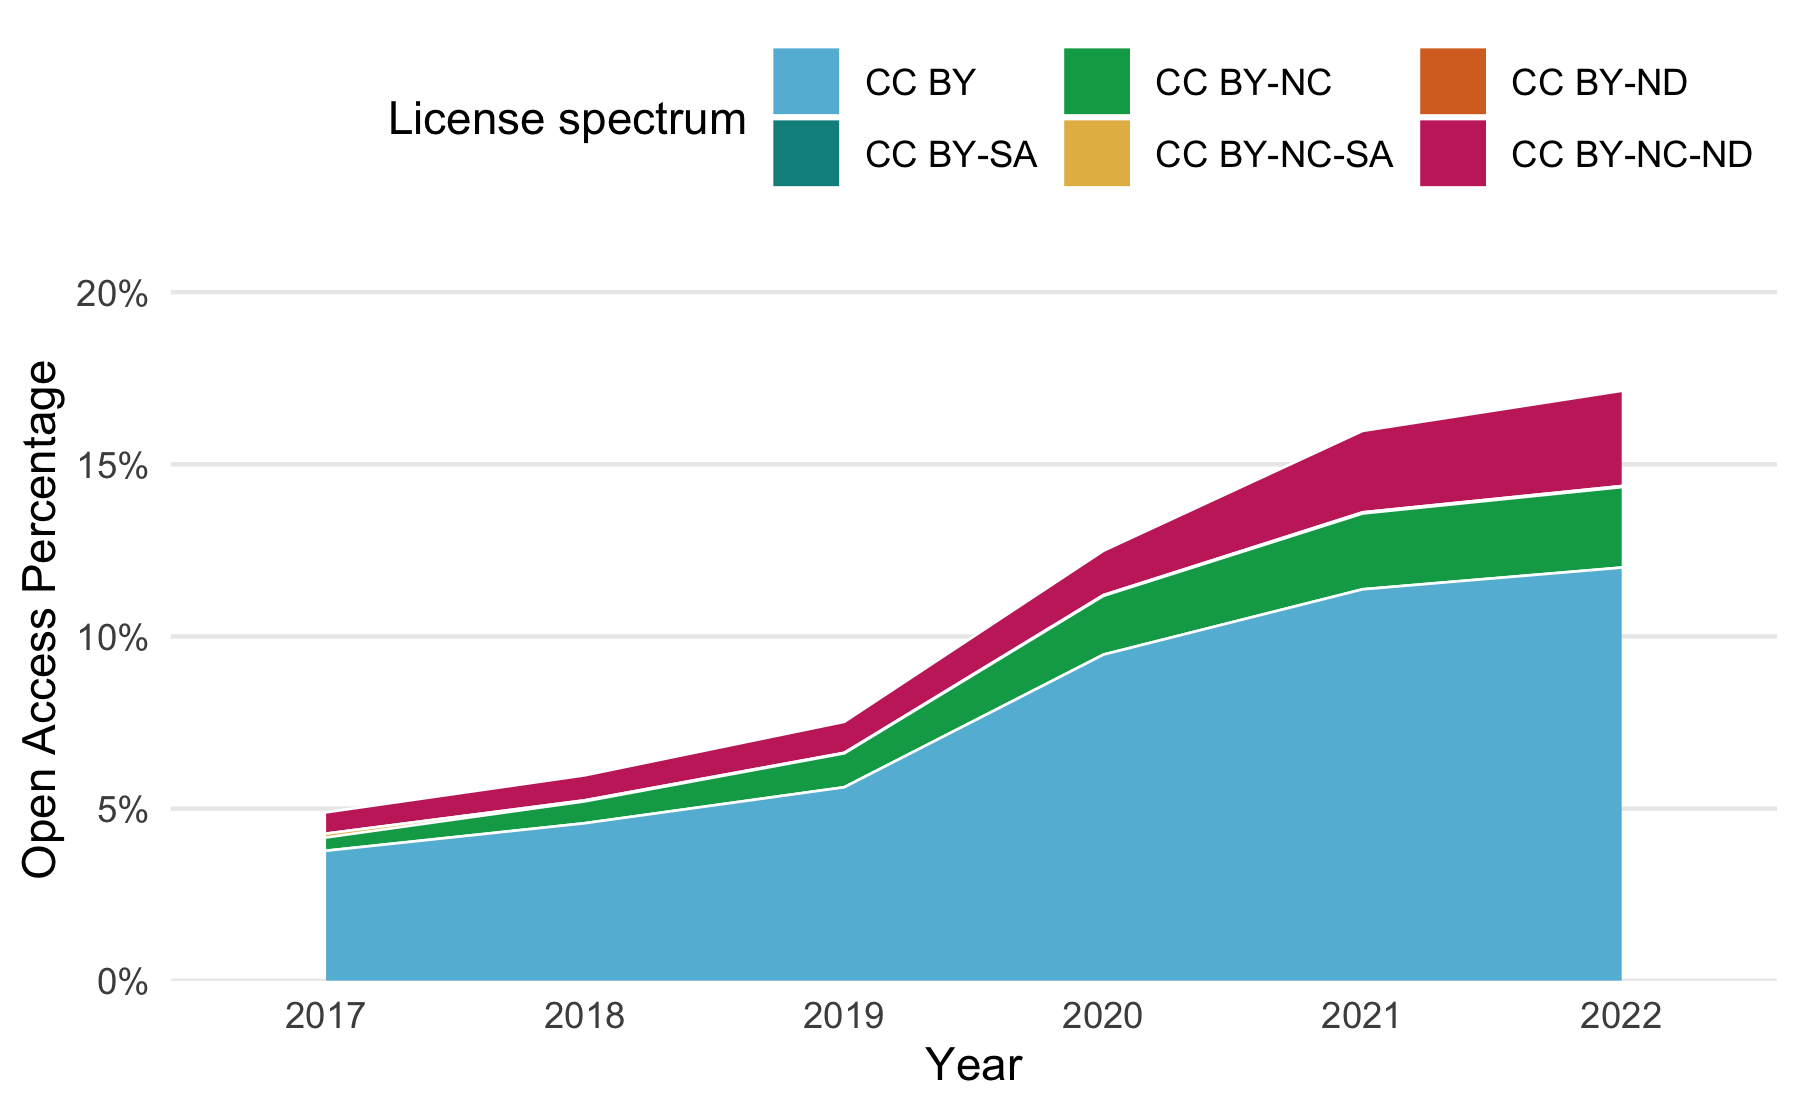
\includegraphics{fig/fig_1.png}
\caption{Relative Entwicklung des globalen
Open-Access-Anteils in hybriden Journalen, welche durch konsortiale
Transformationsverträge in Deutschland mit kommerziellen Verlagen
abgedeckt sind. Datenquellen: Pollack et al.~(2022) und Crossref
(Datenstand März 2022).}
\end{figure}

Abbildung 1 zeigt die prozentuale Entwicklung des Open-Access-Anteils in
hybriden Journalen, welche durch konsortiale Transformationsverträge in
Deutschland abgedeckt sind. Es zeigt sich, dass trotz der gestiegenen
Bedeutung von Open-Access-Transformationsverträgen nur jeder sechste
Artikel in diesen Journalen Open Access publiziert wurde. Ein Großteil
der Artikel wurde unter der Variante CC BY veröffentlicht, welche im
Vergleich zu den anderen Varianten eine umfassende Nachnutzung
ermöglicht.

\begin{figure}
\centering
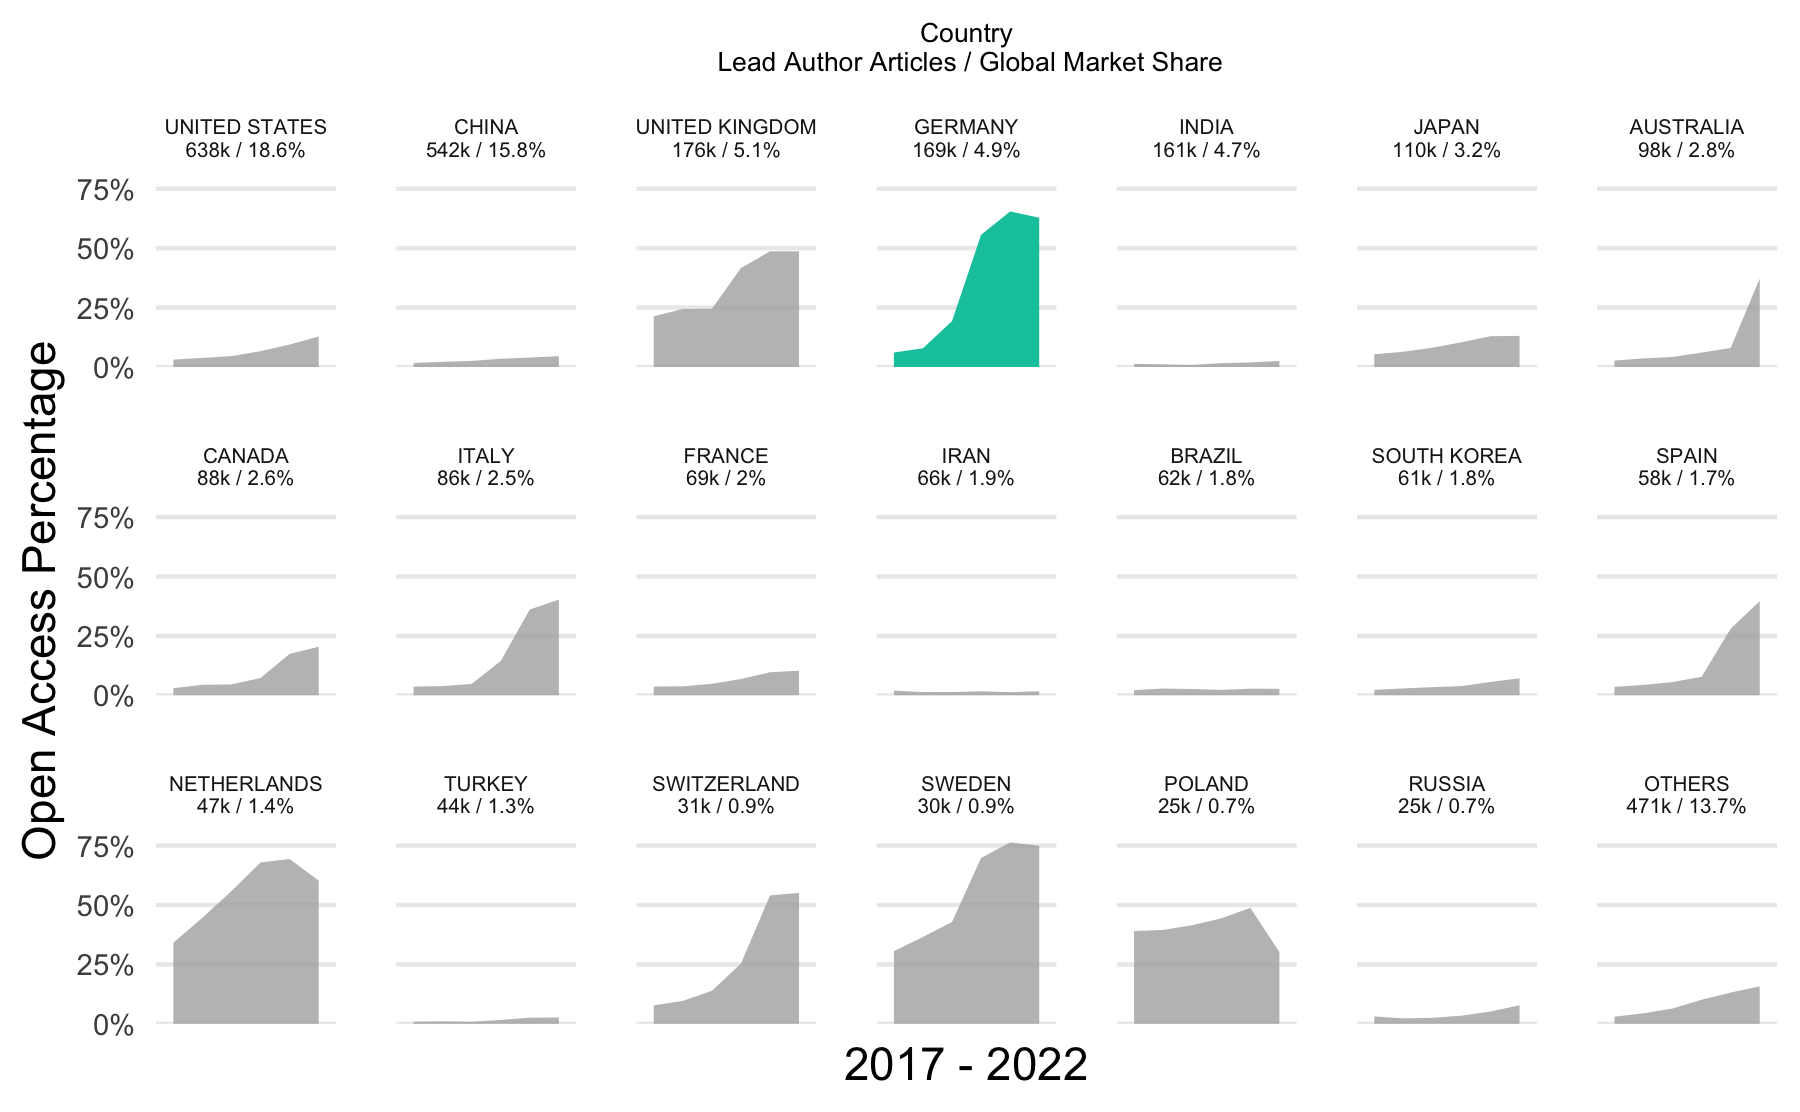
\includegraphics{fig/fig_2.png}
\caption{Relative Entwicklung des Open-Access-Anteils in
hybriden Journalen, welche durch konsortiale Transformationsverträge in
Deutschland mit kommerziellen Verlagen abgedeckt sind je Land.
Abgebildet sind die 20 publikationsstärksten Länder. Länderspezifische
Zwischenüberschriften beinhalten die Gesamtzahl der Publikationen im
Zeitraum sowie deren prozentualer Anteil am untersuchten
Gesamtpublikationsvolumen. Datenquellen: Pollack et al.~(2022), Crossref
und OpenAlex.*}
\end{figure}

Abbildung 2 zeigt den Open-Access-Anteil für die zwanzig
publikationsstärksten Länder gemessen an der Adresse der Erstautor*innen
(\emph{lead author}) und liefert damit ein Indiz, warum Open Access im
hybriden Portfolio der konsortialen Transformationsverträge in
Deutschland weiterhin eine Ausnahme darstellt. Der OA-Anteil in den
publikationsstarken Ländern USA und China ist aufgrund fehlender
nationaler Open-Access-Vereinbarungen weitaus geringer im Vergleich zu
den europäischen Ländern Deutschland, Großbritannien, den Niederlanden
oder Schweden. Die Abbildung zeigt zudem den geringen Open-Access-Anteil
in den asiatischen Ländern Japan und Südkorea oder bei Middle Income
Countries (MICs) wie Indien, Brasilien, Türkei oder Iran. Interessant
ist, dass der Open-Access-Anteil deutscher Artikel im Jahr 2021 trotz
umfangreicher Transformationsverträge bei unter 70\,\% lag.

\hypertarget{diskussion-und-ausblick}{%
\section{Diskussion und Ausblick}\label{diskussion-und-ausblick}}

Ein Cloud-basiertes Hosting von frei verfügbaren Big Scholarly Data
ermöglicht uns unabhängig von Data-Analytics-Angeboten
wissenschaftlicher Verlage umfassende Analysen der Wandlungsprozesse des
wissenschaftlichen Publizierens. Damit machen wir uns nicht nur vom
Datentracking der Anbieter unabhängig (Lauer, 2022), sondern können
zugleich alternative und offene Data-Analytics-Angebote entwickeln.

Nichtsdestotrotz spielen Fragen der Datenabdeckung und -qualität offener
Daten über wissenschaftliche Veröffentlichungen eine wesentliche Rolle.
Wir adressieren dieses Spannungsfeld zum einen über die Beteiligung an
Abdeckungsanalysen im Kontext unserer Mitgliedschaft im Kompetenzzentrum
Bibliometrie\footnote{\url{https://www.bibliometrie.info/}}. Zum anderen
sehen wir im Sinne der ESAC Guidelines\footnote{\url{https://esac-initiative.org/about/transformative-agreements/guidelines-for-transformative-agreements/}}
Wissenschaftliche Bibliotheken in der Verantwortung, auf umfangreiche
und qualitätsbewusste Metadaten bei Verlagen (nicht nur) im Kontext von
Open-Access-Transformationsverträgen hinzuwirken (Geschuhn und Stone,
2017, Voigt, 2020). Zur Unterstützung der Metadatenüberprüfung stellen
wir mit metacheck\footnote{\url{https://subugoe.github.io/metacheck/}}
ein frei verfügbares Werkzeug bereit.

Mittlerweile nutzen wir unser Data Warehouse, das auf BigQuery basiert,
umfangreich in unseren Projekten und für wissenschaftliche
Publikationsvorhaben. Der größte Pluspunkt ist die hohe
Leistungsfähigkeit von BigQuery. Dass komplexe Abfragen von Datensätzen,
deren Dateigrößen im Bereich einer zwei- bis dreistelligen Anzahl
Gigabytes liegen, innerhalb von Sekunden Ergebnisse liefern, ist
großartig und sehr komfortabel. Etwas Vergleichbares könnten wir mit
einer selbst gehosteten Datenbank nicht erreichen. Zudem können wir
Kolleg*innen aus externen Einrichtungen Zugriff auf die Datenbank geben,
etwa im erweiterten Kontext der ESAC Data Analytics Group\footnote{\url{https://esac-initiative.org/about/data-analytics/esac-data-working-group}}
oder des Kompetenzzentrums Bibliometrie. Dank der anstehenden Migration
in einen institutionellen Account unserer Universität durch eine
Rahmenvereinbarung verbessern wir zudem die organisatorische Einbindung
der dienstlichen Nutzung des Cloud-basierten Data Warehouse.

International ist zu beobachten, dass BigQuery in vergleichbaren
Zusammenhängen genutzt wird. Insbesondere die australische Curtin Open
Knowledge Initiative (COKI)\footnote{\url{https://openknowledge.community/}}
mit ihren frei verfügbaren Workflows zur Integration von Big Scholarly
Data in BigQuery ist für uns vorbildlich.\footnote{\url{https://academic-observatory-workflows.readthedocs.io/en/latest/}}
Es stellt sich daher zukünftig die Frage nach Kooperation und Synergien
bezüglich der Bereitstellung und Analyse offener Daten über
wissenschaftliche Veröffentlichungen mittels BigQuery.

\hypertarget{literatur}{%
\section{Literatur}\label{literatur}}

Geschuhn, Kai und Graham Stone. \enquote{It's the Workflows, Stupid!
What Is Required to Make \enquote*{Offsetting} Work for the Open Access
Transition}. \emph{Insights the UKSG Journal} 30, Nr. 3 (8. November
2017): 103--14. \url{https://doi.org/10.1629/uksg.391}.

Hobert, Anne, Najko Jahn, Philipp Mayr, Birgit Schmidt und Niels
Taubert. \enquote{Open Access Uptake in Germany 2010--2018: Adoption in
a Diverse Research Landscape}. \emph{Scientometrics} 126, Nr. 12 (2021):
9751--77. \url{https://doi.org/10.1007/s11192-021-04002-0}.

Jahn, Najko, Maximilian Held, Henrieke Walter, Nick Haupka und Kristine
Hillenkötter. \enquote{HOAD: Data Analytics für mehr Transparenz bei
Open-Access-Transformationsverträgen}. \emph{ABI Technik} 42, Nr. 1
(2022): 64--69. \url{https://doi.org/10.1515/abitech-2022-0007}.

Jahn, Najko, Anne Hobert und Nick Haupka. \enquote{Entwicklung und
Typologie des Datendiensts Unpaywall}. \emph{Bibliothek Forschung und
Praxis} 45, Nr. 2 (2021): 293--303.
\url{https://doi.org/10.1515/bfp-2020-0115}.

Lauer, Gerhard. \enquote{Datentracking in den Wissenschaften}.
\emph{o-bib. Das offene Bibliotheksjournal} 9, Nr. 1 (2022).
\url{https://doi.org/10.5282/O-BIB/5796}.

Pollack, Philipp, Barbara Lindstrot, Irene Barbers und Franziska
Stanzel. \enquote{Open Access Monitor: Zeitschriftenlisten}. Jülich
DATA, 2022. \url{https://doi.org/10.26165/JUELICH-DATA/VTQXLM}.

Voigt, Michaela. \enquote{DEAL Open-Access-Option optimal nutzen -- ein
Bibliothekspraxisbericht}, LIBREAS.Library Ideas, 38 (2020).
\url{https://libreas.eu/ausgabe38/voigt/}.

Wickham, Hadley und Jennifer Bryan. \emph{bigrquery: An Interface to
Google's \enquote{BigQuery} \enquote{API}} (R package version 1.4.0),
2021.
\href{https://cran.r-project.org/package=bigrquery}{https://CRAN.R-project.org/package=bigrquery}.

%autor
\begin{center}\rule{0.5\linewidth}{0.5pt}\end{center}

\textbf{Nick Haupka}, \textbf{Najko Jahn} und \textbf{Dr.~Anne Hobert}
arbeiten an der Niedersächsischen Staats- und Universitätsbibliothek
(SUB) in der Gruppe Wissen als Gemeingut und sind dort mit Datenanalysen
im Kontext Wissenschaftlicher Information betraut. Mehr Infos:
\url{https://subugoe.github.io/scholcomm_analytics/about.html}

\end{document}
